\section{Interpolation with Rational Functions}

\textbf{(a)}

For a fixed degree \(m\), the interpolation condition is
\[
    y_i =
    \frac{a_0+a_1x_i+\cdots+a_mx_i^m}
    {1+b_1x_i+\cdots+b_mx_i^m}.
\]
Multiplying by the denominator gives
\[
    a_0+a_1x_i+\cdots+a_mx_i^m
    -y_i b_1x_i-\cdots-y_i b_mx_i^m
    =
    y_i.
\]
This is linear in the unknown coefficients
\[
    \theta =
    \begin{bmatrix}
        a_0&a_1&\cdots&a_m&b_1&\cdots&b_m
    \end{bmatrix}^T.
\]
So for each \(m=0,1,2,\ldots\), we form the linear system
\[
    \begin{bmatrix}
        1 & x_i & \cdots & x_i^m
        & -y_i x_i & \cdots & -y_i x_i^m
    \end{bmatrix}
    \theta
    =
    y_i,
    \qquad i=1,\ldots,N.
\]
The smallest degree \(m\) is the first value for which this system is
consistent and the resulting rational function has degree \(m\).

\textbf{(b)}

\begin{figure}[h]
    \centering
    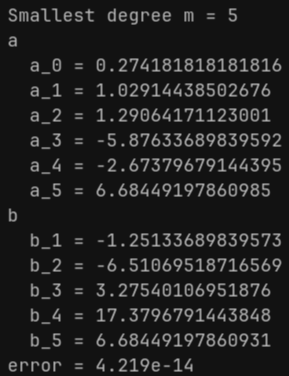
\includegraphics[width=0.3\textwidth]{img/8b.png}
\end{figure}

\begin{figure}[H]
    \centering
    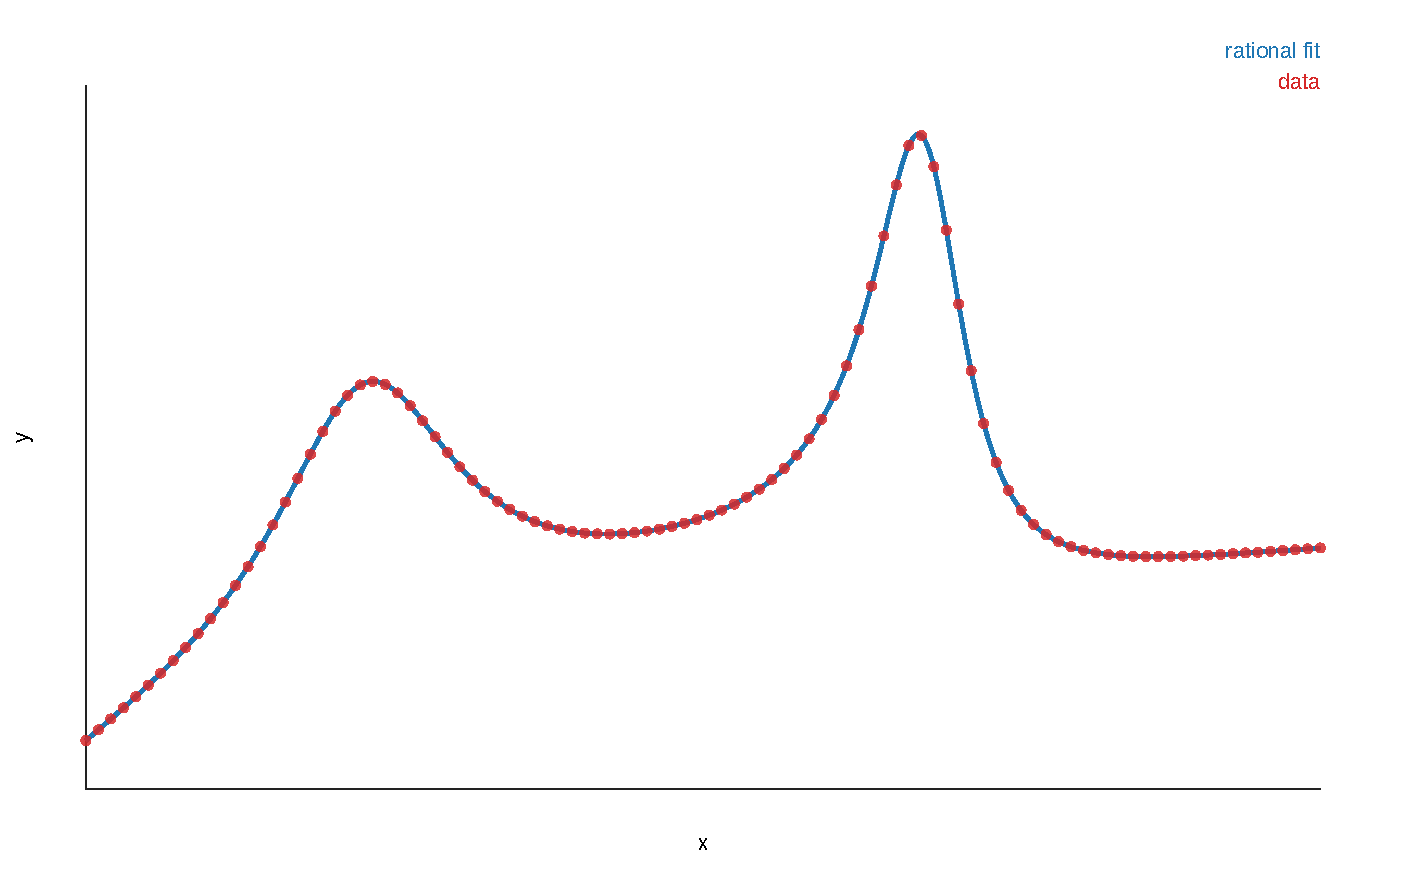
\includegraphics[width=0.85\textwidth]{img/p8_rational_interpolation.pdf}
    % \caption{Rational interpolant and data points for problem 8.}
\end{figure}

\begin{lstlisting}
using LinearAlgebra
using JSON3
using Printf

data_file = joinpath(@__DIR__, "rational_interpolation_data.json")
data = JSON3.read(read(data_file, String))
x = Float64.(data.x.data)
y = Float64.(data.y.data)

function interpolation_matrix(x, y, m)
    numerator_terms = [x .^ j for j in 0:m]
    denominator_terms = [-(y .* (x .^ j)) for j in 1:m]
    return hcat(numerator_terms..., denominator_terms...)
end

function rational_value(x, a, b)
    numerator = sum(a[j + 1] * x^j for j in 0:(length(a) - 1))
    denominator = 1.0 + sum(b[j] * x^j for j in 1:length(b))
    return numerator / denominator
end

for m in 0:div(length(x) - 1, 2)
    A = interpolation_matrix(x, y, m)
    theta = A \ y
    residual = norm(A * theta - y, Inf)

    if residual <= 1e-8
        a = theta[1:(m + 1)]
        b = theta[(m + 2):end]
        yhat = [rational_value(xi, a, b) for xi in x]

        max_error = norm(yhat - y, Inf)

        break
    end
end
\end{lstlisting}